\begin{figure}[t]
\begin{minipage}[b]{0.49\linewidth}
\centering
\footnotesize
\begin{lstlisting}[language=Java,basicstyle=\scriptsize\ttfamily]
public static void testMethod1(int x) {
 if(Verify.getBoolean()) {
  if(Verify.getBoolean()) {
   if(x <= 60)
    ...println("success");
   else
    assert false;
  } else {
   if(x <= 30)
    ...println("success");
   else
    assert false;
  }
 } else {
  if(x <= 55)
   ...println("success");
  else
   assert false;
 }
}
\end{lstlisting}
\end{minipage}%
\begin{minipage}[b]{0.49\linewidth}
\centering
\tikzstyle{gn} = [circle, fill=gray!20, draw]
\tikzstyle{wn} = [circle, draw]
\tikzstyle{bn} = [text width=2em, text centered]
\tikzstyle{every node}=[font=\scriptsize, inner sep=0pt, minimum size=0.4cm]
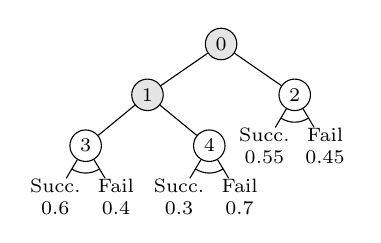
\begin{tikzpicture}[scale=0.38, level/.style={sibling distance = 15mm, level distance = 17mm}]
  \node[gn] {0}
   child{
    node[gn,xshift=-6.5mm] {1}
     child{
      node[wn,xshift=-5mm] {3}
       child{
        node[bn,xshift=-1mm] {Succ. 0.6}
        edge from parent coordinate[midway](m1)
       }
       child{
        node[bn,xshift=1mm] {Fail 0.4}
        edge from parent coordinate[midway](m2)
       }
      edge from parent
     }
     child{
      node[wn,xshift=5mm] {4}
       child{
        node[bn,xshift=-1mm] {Succ. 0.3}
        edge from parent coordinate[midway](m3)
       }
       child{
        node[bn,xshift=1mm] {Fail 0.7}
        edge from parent coordinate[midway](m4)
       }
      edge from parent
     }
   }
   child{
    node[wn,xshift=6.5mm] {2}
     child{
      node[bn,xshift=-1mm] {Succ. 0.55}
      edge from parent coordinate[midway](m5)
     }
     child{
      node[bn,xshift=1mm] {Fail 0.45}
      edge from parent coordinate[midway](m6)
     }
    edge from parent
   }
;
\draw (m1) to[bend right] (m2);
\draw (m3) to[bend right] (m4);
\draw (m5) to[bend right] (m6);
\end{tikzpicture}
\end{minipage}
\caption{Example 1}
\label{fig:example}
\end{figure}

